\section{Process}

\pagebreak
\section{Model}
\subsection{Overview}
Persons that most likely will use the website
\begin{itemize}
	\item Current students
	\item Potential students
	\item Industry partners
\end{itemize}

\begin{center}
	
\begin{scaletikzpicturetowidth}{\textwidth}
	\begin{tikzpicture}[scale=\tikzscale,
	level distance=5cm]
	
	\Tree[.{Most likely users of website}  
	\edge node{} ; [.{Current students}  
		\edge node{} ; [.{Personae 1} 
			\edge node{} ; [.{Scenario 1} ] 
			\edge node{} ; [.{Scenario 2} ] 
			\edge node{} ; [.{Scenario 3} ] 
			 ] ] 
	\edge node{}; [.{Potential students}    
		\edge node{} ; [.{Personae 2} 
			\edge node{} ; [.{Scenario 1} ] 
			\edge node{} ; [.{Scenario 2} ] 
			\edge node{} ; [.{Scenario 3} ] 
		] 
	] 
	\edge node{}; [.{Industry partners}   
		\edge node{} ; [.{Personae 3} 
			\edge node{} ; [.{Scenario 1} ] 
			\edge node{} ; [.{Scenario 2} ] 
			\edge node{} ; [.{Scenario 3} ] 
		] 
	]
	]

%\Tree[.{Most likely users of website}
%\edge node[midway,left] {false}; [.{Current students}]
%\edge node[midway,right] {true}; [.{Potential students}]
%]
	
	\end{tikzpicture}
\end{scaletikzpicturetowidth}
\end{center}



\pagebreak
%
%\subsection{Personae}
%\subsubsection{Persona1 (Current student)}
%\begin{itemize}
%	\item 21 years old
%	\item 2nd year CompScience student
%	\item Likes using command line for simplest stuff
%	\item Has blue long hair
%	\item In his spare time he writes javascript apps that noone besides him will ever use
%\end{itemize}
%
%\pagebreak
%\subsubsection{Persona2 (Potential student)}
%\begin{itemize}
%	\item 17 years old
%	\item She is good in math but would also like to do something social
%	\item Her friends are all very girly
%	\item She plays football
%	\item She spends her evenings on facebook
%\end{itemize}
%
%\pagebreak
%\subsubsection{Persona3 (Industry partners)}
%\begin{itemize}
%	\item Working at some big software company
%	\item Has already 20 years of professional experience
%	\item Wants to find out new ways of doing a task
%	\item Company can't afford own research
%\end{itemize}
%
%\pagebreak

\subsubsection{Persona 1: Kenneth Smith}
%Intro: 
Kenneth (Kenny) Smith is a 3rd year Computer Science student at Victoria University of Wellington. He is a hard worker and prides himself on his high level of achievement across his courses. He's always had a passion for computers and from a young age was interested in coding using basic applications like Scratch and getting involved with Coding workshops and camps. This is partially due to his Parents both working in development fields. When he isn't studying, Kenny is often gaming. He plays League of Legends, World of Warcraft and Counter Strike GO and often plays online with his friend group. He has played and love heavy metal guitar since he was 10, but has not maintained his abilities since his focus is now on University work. He also has a long distance girlfriend that he has been with for 2 years. He sometimes struggles to balance his studying, gaming and girlfriend. He has a life goal of getting a high paying and stimulating job in the computer science field. 

\begin{figure}[h]
	\centering
	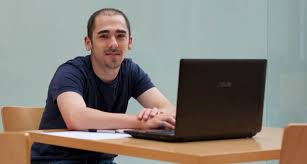
\includegraphics[width = 0.25\textwidth]{images/index.jpg}
\end{figure}
\noindent
\textbf{Personal: }\\
\begin{tabularx}{\textwidth}{l X}
	Name & Kenny\\
	Age & 21\\
	Gender & Male\\
	Education & NCEA Level 3 with Excellence Endorsed (Maths, Chemistry, Digital Technology and Music)\\
	Spare time & PC Gamer (League of Legends, Counter Strike, WoW)\\
	& Heavy metal guitar enthusiast (both plays and listen)\\
	& long distance girlfriend\\
	Attitudes & Considers himself a realist, is more likely a pessimist. Likes to think he knows more than others. Prides himself on his computer abilities so is particularly short tempered  if he is struggling to achieve easy tasks on the computer\\
	Aptitudes & Kenny is intelligent and good at abstract thought.\\
	Skills & Competent with computers, studying, playing guitar and gaming.\\
	Motivations & Enjoys learning new things, as long as they are not too hard. 
	
\end{tabularx}
\noindent
\textbf{Technical: }\\
\begin{tabularx}{\textwidth}{l X}
General & Kenny is a strict windows user. His main device is his desktop gaming PC (his pride and joy). If he is using the Web, it is done usually through his PC. He doesn't prioritize his cell phone for anything other than calling and messaging.  He spends most of his time on his PC, often using Google chrome for the internet, IDE softwares for coding and Steam for his gaming. \\

Domain Knowledge& Confident with terminology and details of the Engineering and Computer Science degree.\\

System Knowledge& Has used the ecs website occasionally but often just Googles to get straight to where he needs to be. \\

Computer self efficacy& Kenny has high confidence in achieving computing tasks, to the point that he is infuriated if he cant achieve his goal with ease. He rarely blames himself for problems he's having with technology. \\

Information Processing& He likes to find the answer to his queries the fastest way possible. Avid stack-overflow user. He does not enjoy sourcing information from a number of webpages/websites. If there are a number of answers he will choose the shortest.\\

Tinkering& Kenny loves tinkering with new programs and new features of software he currently uses. He will tinker away for a long time before Googling for help. He has never considered using built in help menus. \\

Quote& "Which under qualified fool designed this [ecs-vuw] site?! It shouldn't be this difficult to find the course requirements for my next semester courses".
\end{tabularx}

\pagebreak

\subsection{Scenarios}

\begin{itemize}
	\item asdf
\end{itemize}

\begin{enumerate}
	\item asdf
\end{enumerate}